\documentclass[tufte-handout]{standalone}
\usepackage{mathpazo} % Sets Palatino as the main font
\usepackage{tikz}
\usetikzlibrary{shadings,3d,angles,quotes,calc,backgrounds,decorations.markings}

% Define colors
\definecolor{darkslategray}{rgb}{0.18, 0.31, 0.31}
\definecolor{myorange}{rgb}{0.89804, 0.55686, 0.19608}

\tikzstyle{title} = [rectangle, rounded corners, minimum width=3cm, minimum height=0.5cm, text centered, fill=myorange!20, draw=myorange!80!black, font=\bfseries] 


\begin{document}

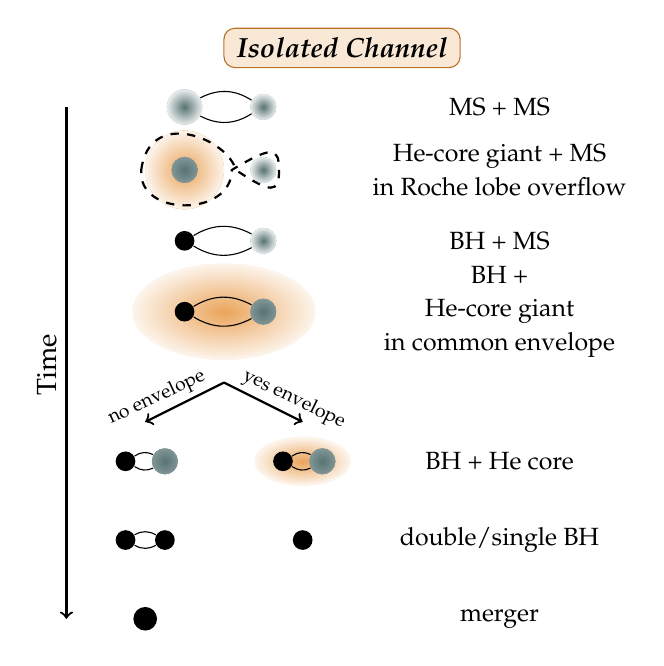
\begin{tikzpicture}
% Time arrow

    \node at (2., 7.25) [title]{\itshape Isolated Channel};
    
    \draw[thick,->] (-1.5,6.5) -- (-1.5,0) node[midway,left,rotate=90, yshift=0.25cm,xshift=0.5cm] {Time};

    % Stage 1: MS + MS
    \node (ms1) at (0,6.5) [circle, fill=darkslategray!60, minimum size=0.45cm,, inner sep=0,shading=radial,inner color=darkslategray!80, outer color=darkslategray!10] {};
    \node (ms2) at (1,6.5) [circle, fill=darkslategray!60, minimum size=0.3cm, shading=radial, inner color=darkslategray!80, outer color=darkslategray!10] {};
    \draw (ms1) to[bend left=30] (ms2);
    \draw (ms2) to[bend left=30] (ms1);
    \node at (4,6.5) [align=center] {\small MS + MS};


    % Stage 2: Roche Lobe Overflow (He-core GIANT + MS with Figure-8)
    \node (giant) at (0,5.7) [circle, fill=myorange, minimum size=1.cm, shading=radial, inner color=myorange!80, outer color=myorange!10] {};
    \node (ms3) at (1,5.7) [circle, fill=darkslategray!60, minimum size=0.3cm, shading=radial, inner color=darkslategray!80, outer color=darkslategray!10] {};
    \node (ms3a) at (0,5.7) [circle, fill=darkslategray!60, minimum size=0.1cm, shading=radial, inner color=darkslategray!80, outer color=darkslategray!60] {};

    % Roche Lobe (Figure-8) 
    \draw[dashed, thick]
        (-0.55,5.7) .. controls (-0.45,6.5) and (0.55,6.1) .. (0.65,5.7)  % Left lobe
        .. controls (1.1,5.4) and (1.2,5.4) .. (1.2,5.7) % Smooth connection
        .. controls (1.2,6) and (1.1,6) .. (0.6,5.7)  % Right lobe
        .. controls (0.6,5.1) and (-0.6,5.1) .. (-0.55,5.7);

        
    \node at (4,5.7) [align=center] {\small He-core giant + MS \\ \small in Roche lobe overflow};

    % Stage 3: BH + MS
    \node (bh1) at (0,4.8) [circle, fill=black, minimum size=0.25cm, inner sep=0] {};
    \node (ms4) at (1,4.8) [circle, fill=darkslategray!60, minimum size=0.3cm, shading=radial, inner color=darkslategray!80, outer color=darkslategray!10] {};
    \draw (bh1) to[bend left=30] (ms4);
    \draw (ms4) to[bend left=30] (bh1);
    \node at (4,4.8) [align=center] {\small BH + MS};

    % Stage 4: Common Envelope Phase
    \draw[thick, myorange!10,shading=radial, inner color=myorange!80, outer color=myorange!10] (0.5,3.9) ellipse (1.15cm and 0.6cm); % Common Envelope Bubble
    \node (bh2) at (0,3.9) [circle, fill=black, minimum size=0.25cm, inner sep=0] {};
    \node (giant2) at (1,3.9) [circle, fill=darkslategray!60, minimum size=0.3cm, shading=radial, inner color=darkslategray!80, outer color=darkslategray!60] {};
    \draw (bh2) to[bend left=30] (giant2);
    \draw (giant2) to[bend left=30] (bh2);    
    \node at (4,3.9) [align=center] {\small BH + \\ \small He-core giant \\ \small in common envelope};

    
    % Arrows for decision paths
    \draw[->, thick] (0.5,3) -- (-0.5,2.5) node[midway, left, rotate=25, yshift=0.2cm,xshift=0.5cm] {\scriptsize no envelope};
    \draw[->, thick] (0.5,3) -- (1.5,2.5) node[midway, right,rotate=-26, yshift=0.2cm,xshift=-0.5cm] {\scriptsize yes envelope};

    % Outcome 1: BH + BH (YES branch)
    \node (bh3) at (-0.75,2) [circle, fill=black, minimum size=0.25cm, inner sep=0] {};
    \node (bh4) at (-0.25,2) [circle, fill=darkslategray!60, minimum size=0.3cm, shading=radial, inner color=darkslategray!80, outer color=darkslategray!60] {};
    \draw (bh3) to[bend left=30] (bh4);
    \draw (bh4) to[bend left=30] (bh3);

    \node (bh3a) at (-0.75,1) [circle, fill=black, minimum size=0.25cm, inner sep=0] {};
    \node (bh4a) at (-0.25,1) [circle, fill=black, minimum size=0.25cm, inner sep=0] {};
    \draw (bh3a) to[bend left=30] (bh4a);
    \draw (bh4a) to[bend left=30] (bh3a);

    % Outcome 2: Single BH left (NO branch)
    \draw[thick, myorange!10,shading=radial, inner color=myorange!80, outer color=myorange!10] (1.5,2) ellipse (0.6cm and 0.3cm); % Common Envelope Bubble
    \node (bh5) at (1.25,2) [circle, fill=black, minimum size=0.25cm, inner sep=0] {};
    \node (hecore) at (1.75,2) [circle, fill=darkslategray!60, minimum size=0.3cm, shading=radial, inner color=darkslategray!80, outer color=darkslategray!60] {};
    \draw (bh5) to[bend left=30] (hecore);
    \draw (hecore) to[bend left=30] (bh5);
    \node at (4,2) [align=center] {\small BH + He core};
    

    % Merger (Final Stage)
    \node (bh6) at (-0.5,0) [circle, fill=black, minimum size=0.3cm, inner sep=0] {};
    \node at (4,0) [align=center] {\small merger};

    \node (bh6a) at (1.5,1) [circle, fill=black, minimum size=0.25cm, inner sep=0] {};
    \node at (4,1) [align=center] {\small double/single BH};


\end{tikzpicture}

\end{document}
